\section{Learning the Pareto-optimal Set Efficiently }
\label{sec:learn-pareto-optim}

In this section, we discuss techniques that learns the Pareto-optimal set
efficiently. We first describe our programming abstraction and profiling
formalism. We then focus on addressing two profiling challenges: the large
parameter space and device heterogeneity. $(i)$ We propose to use Bayesian
Optimization (BO) to address large parameter space with multiple parameters. And
we show that it outperforms previous approaches (random search and coordinate
search). $(ii)$ We propose to use profile transfer to derive the profile for a
new device without running expensive profiling from scratch.

\subsection{Programming Abstraction for Compute Adaptation}
\label{sec:progr-abstr}

Unlike \autoref{sec:structure-adapt}, the algorithms and parameters do not come
from a series of chained operators. Therefore, we need new programming
abstractions here. However, the design goal is similar: to free developers from
specifying exact rules and allow specifications with options.

We use \texttt{trait}\footnote{\texttt{trait} in Rust is similar to
  \texttt{interface} in other languages.} to abstract each algorithm, as below:

\begin{lstlisting}[xleftmargin=.1\textwidth, xrightmargin=.1\textwidth, language=Rust]
trait Algorithm {
    type I;
    type O; 
    type P;
    fn execute(&mut self, i: &Self::I, p: &Self::P) -> Self::O;
}
\end{lstlisting}

Each algorithm is specified by its input data type \texttt{I}, output data type
\texttt{O}, a parameter type \texttt{P}, and its behavior function
\texttt{execute}. For any data type \texttt{T} that implements
\texttt{Algorithm} trait, the function \texttt{execute} can access the internal
data structure of \texttt{T} in a mutable way: \texttt{\&mut self}. Type
\texttt{I}, \texttt{O}, and \texttt{P} are abstract types and the implementation
must specify the concrete types. We show an implementation of Viola-Jones in
\autoref{fig:vj} where the input type is an image, the output type is a
detection, and the parameter is \texttt{VJParameters}.

For tunable parameters, we need to be able to specify at least three parts:
\texttt{min}, \texttt{max}, and \texttt{step}. We extend an algorithm's
parameter by augmenting it with annotations. In Rust, this can be implemented
with procedural macros as a syntax extension. \autoref{fig:vj} shows these
annotation in blue: we use \texttt{\#[derive(Adapt)]} to mark that this
\texttt{struct} is a tunable parameter and use \texttt{\#[adapt(...)]} to mark
its field.

\begin{figure}
  \centering
\begin{lstlisting}[language=Rust]
#[derive(Adapt)]
struct VJParameters {
    #[adapt(min = "0", max = "20", step = "1")]
    min_neighbors: i64,

    #[adapt(min = "0", max = "190", step = "10")]
    min_size: i64,

    #[adapt(min = "1.01", max = "1.5", step = "0.01")]
    scale_factor: f64,
}

struct VJ {
  // ... omitted ...
}

impl Algorithm for VJ {
    type I = Image;
    type O = Detection;
    type P = VJParameters;

    fn execute(&mut self, image: &Image, opt: &VJParameters) -> Detection {
        // ... omitted ...
    }
}
\end{lstlisting}
  \caption{Viola-Jone face detector parameters \texttt{VJParameters} annotated
    with adaptation. \texttt{VJ} implements the \texttt{Algorithm} trait.}
  \label{fig:vj}
\end{figure}

\subsection{Profiling Formalism}
\label{sec:profiling-formalism}

The goal of profiling is to build a profile that charactersizes the tradeoff
between application accuracy and processing times such that for a running
application, it can choose the right algorithm/parameter to meet the
deadline. As discussed in \autoref{sec:perf-model-chall}, we are only interested
in the Pareto-optimal set.

We start with defining the Pareto-optimal set for a specific algorithm with
varying parameters. For an algorithm with $n$ parameters, e.g., $n$ is 3 for
Viola-Jones, we call each parameter a knob and refer it as $k_i$. The
combination of all knobs forms a parameter \textit{configuration}
$c = [k_{1}, k_{2}, ... k_{n}]$. The set of all possible configurations
$\mathbb{C}$ is the space that the profiling explores for this algorithm. For
each configuration $c$, we are interested in two mappings: a mapping from $c$ to
its processing times $T(c)$ and its accuracy measure $A(c)$.  The profiling
looks for Pareto-optimal configurations; that is, for any configuration $c$ in
the Pareto-optimal set $\mathbb{P}$, there is no alternative configuration $c'$
that requires a smaller processing time and offers a higher accuracy. Formally,
$\mathbb{P}$ is defined as follows:

{\small \vspace{-1em}
  \begin{equation}
    \mathbb{P} = \{ c \in \mathbb{C} : \{ c' \in \mathbb{C}: T(c') < T(c),
    A(c') > A(c) \} = \varnothing\}
  \label{eq:pareto2}
\end{equation}
}%

Once we have the Pareto-optimal set for one algorithm, we can compose multiple
algorithms and merge their Pareto-optimal set by finding the global
Pareto-optimal configurations. Both processing times and application accuracy
are simply real numbers and can be compared, despite each algorithm's parameters
may be completely different.

\subsection{Profiling Parameters with Bayesian Optimization}
\label{sec:prof-param-with}

Bayesian Optimization (BO)~\cite{snoek2012practical} is a technique that
approximates black-box functions with proxy functions, iteratively proposes new
sample point to evaluate in the large parameter space, and finds the global
maximum (or minimum). It is effective for black-box functions when evaluating
each sample is expensive and noisy, such as tuning parameters and model
hyperparameters in ML tasks~\cite{snoek2012practical}. A comprehensive review of
BO is beyond the scope of this thesis. We briefly describe what BO brings using
an example without going into the gory details.

\begin{figure}
  \begin{subfigure}{\textwidth}
    \centering
    
\includegraphics[width=0.5\textwidth]{figures/bo-legend.pdf}
  \end{subfigure}
  \vspace{0.2em}
  \\
  \centering
  \begin{subfigure}{0.45\textwidth}
    \centering
    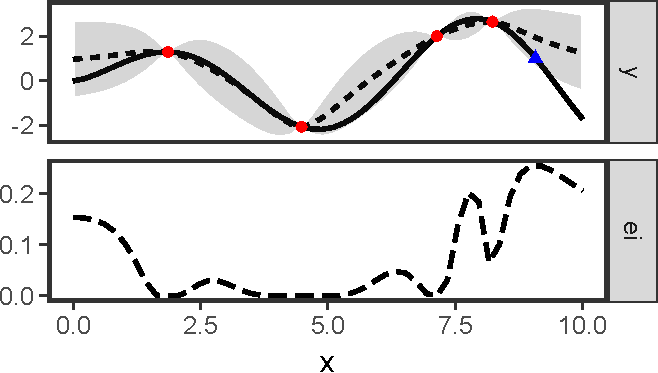
\includegraphics[width=\textwidth]{figures/bo1.pdf}
    \caption{First Iteration.}
  \end{subfigure}
  \hspace{1em}
  \begin{subfigure}{0.45\textwidth}
    \centering
    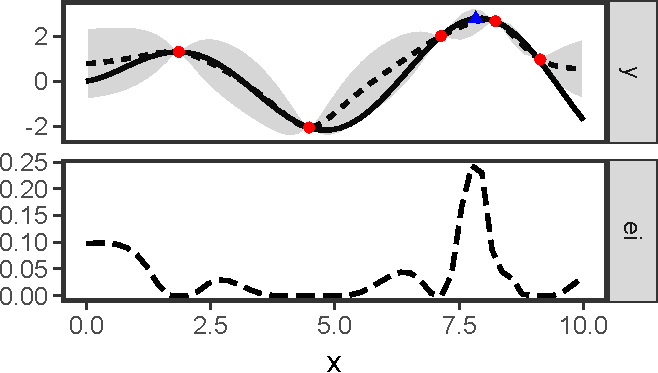
\includegraphics[width=\textwidth]{figures/bo2.pdf}
    \caption{Second Iteration.}
  \end{subfigure}
  \caption{Bayesian Optimization illustrated.}
  \label{fig:bo-1d}
\end{figure}

\autoref{fig:bo-1d} illustrates the process of finding the maximum point for
1-dimension Alpine N. 2 function~\cite{clerc1999swarm} (this figure is produced
with the mlrMBO package~\cite{bischl2017mlrmbo}). The solid line labeled $y$ is
the target black-box function. The red dots represent samples that have been
evaluated. BO reconstructs a function that best fits these observed samples: the
dashed line $\hat{y}$ (yhat) along with the confidence region (in grey shade).
BO then uses an acquisition criteria to determine how to sample the next point.
In this example, we use expected improvement (EI, in long-dashed line) that
balances high objective (exploitation) and high uncertainty
(exploration)~\cite{shahriari2016taking}. The point that maximizes EI is then
proposed as the next sample point (blue triangles). Running this process
iteratively, BO is able to solve the maximization problem of a black-box
function.

% (2.808119, 7.92)

BO recently has gain attraction beyond ML scope.
CherryPick~\cite{alipourfard2017cherrypick} uses BO to find the near-optimal
cloud configurations for big data analytics, i.e., minimizing the cost of
execution. Google uses BO to optimize chocolate chip cookies
recipes~\cite{solnik2017bayesian}, i.e., maximizes the tastiness.

Our problem is more complex as we are solving multi-objective optimizations
(MOO). Specifically, it has two objectives: application accuracy and processing
times. It is trivial to maximize application accuracy or minimize processing
times alone. Previous approaches often transform multiple objectives into a
single objective using scalarization techniques: using weighted sum to combine
different objectives. These approaches are expected to be
suboptimal~\cite{knowles2006parego}. Recent research progress has made the
transformation unnecessary. We can directly consider the Pareto-optimal set and
evaluate the improvements with different acquisition criteria: $(i)$ additive
epsilon~\cite{binoisgpareto}, $(ii)$ hypervolume~\cite{binoisgpareto}; $(iii)$
the entropy of the posterior distribution over the Pareto-optimal
set~\cite{hernandez2016predictive}. We illustrate the first two criteria in
\autoref{fig:bo-2d}. We use PESMO~\cite{hernandez2016predictive} because of its
availability and ease of use. It is available within the Spearmint
package~\cite{snoek2016spearmint}.  PESMO also has a low computational cost: it
grows linearly with respective to the total number of objectives $K$.

\begin{figure}
  \centering
  \begin{subfigure}{0.45\textwidth}
    \begin{tikzpicture}
      \pgfplotstableread{
        0 0.1 -0.1
        0 0.1  0.2
        1 0.25 0.5
        2 0.4  0.6
        3 0.5  0.85
        4 0.9  0.9
        4 1.2  0.9
      }\datatable
      \begin{axis}[
        width  = \textwidth,
        xlabel = Processing Times (normalized),
        ylabel = Accuracy,
        axis line style = thick,
        ymin   = 0,
        ymax   = 1,
        ytick  = {0, 0.2, 0.4, 0.6, 0.8, 1},
        xmin   = 0,
        xmax   = 1,
        xtick  = {0, 0.2, 0.4, 0.6, 0.8, 1},
        ]

        \addplot+[red!50,
        mark size=3pt, mark options={draw=red!0, fill=red!80}, const
        plot mark left, thick] table [x index=1, y index=2]{\datatable};

        \addplot[mark=triangle*, mark options={draw=blue!80, fill=blue!80},
        mark size=3pt, fill=blue!80, only marks]
        coordinates { (0.3, 0.7) };

        \draw[-, blue, dashed] (axis cs:0.3, 0.5) -- (axis cs:0.3, 0.7);
        \draw[-, blue, dashed] (axis cs:0.3, 0.7) -- (axis cs:0.5, 0.7);
        \draw[<->, >=stealth, blue] (axis cs:0.45, 0.6) -- (axis cs:0.45, 0.7);
        \draw[<->, >=stealth, blue] (axis cs:0.3, 0.55) -- (axis cs:0.4, 0.55);

      \end{axis}
    \end{tikzpicture}
  \end{subfigure}
  \hspace{1em}
  \begin{subfigure}{0.45\textwidth}
    \begin{tikzpicture}[
      triangle/.style = {fill=blue!80, regular polygon, regular polygon sides=3}
      ]

      \pgfplotstableread{
        0 0.1 -0.1
        0 0.1  0.2
        1 0.25 0.5
        2 0.4  0.6
        3 0.5  0.85
        4 0.9  0.9
        4 1.2  0.9
      }\datatable
      \begin{axis}[
        width  = \textwidth,
        xlabel = Processing Times (normalized),
        ylabel = Accuracy,
        axis line style = thick,
        ymin   = 0,
        ymax   = 1,
        ytick  = {0, 0.2, 0.4, 0.6, 0.8, 1},
        xmin   = 0,
        xmax   = 1,
        xtick  = {0, 0.2, 0.4, 0.6, 0.8, 1},
        axis on top
        ]

        \addplot+[blue!50, no marks,
        mark size=3pt, mark options={draw=blue!0, fill=blue!80},
        % pattern=north east lines,
        % pattern color=blue!50,
        fill=blue!20,
        ]
        coordinates {(0.3, 0.5) (0.3, 0.7) (0.5, 0.7) (0.5, 0.6) (0.4, 0.6)
          (0.4, 0.5) (0.3, 0.5)};

        \addplot+[red!50, mark=*,
        mark size=3pt, mark options={draw=red!0, fill=red!80}, const
        plot mark left, thick,
        pattern=north west lines,
        pattern color=red!50]
        table [x index=1, y
        index=2]{\datatable} \closedcycle;

        \addplot[mark=triangle*, mark options={draw=blue!80, fill=blue!80},
        mark size=3pt, fill=blue!80, only marks]
        coordinates { (0.3, 0.7) };

      \end{axis}
    \end{tikzpicture}
  \end{subfigure}
  \caption{To find the Pareto-optimal set that maximizes accuracy while
    minimizing processing times, the acquisition criterion can suggest new
    samples (blue triangles) to the current Pareto-optimal set (red points) by
    maximizing additive epsilon (left, blue arrows) or hypervolume (right, blue
    shade area). This illustration is adapted from GPareto
    vignette~\cite{binoisgpareto}.}
  \label{fig:bo-2d}
\end{figure}

%%% Local Variables:
%%% mode: latex
%%% TeX-master: "../compute"
%%% End:


We then show that BO can effectively explore the large design space and come up
with a better Pareto-optimal set. We compare BO with two baseline approaches:
$(i)$ random search; $(ii)$ coordinate search.

For coordinate search, because it is a greedy approach, the original two
objectives is converted into a single objective: $X(c) = A(c) - \beta T(c)$. We
augment the basic version of the coordinate search with a few techniques: $(i)$
to avoid starting with an expensive configuration and exploring its neighbors,
we pick $m$ random configurations and start from the one with the highest
$X$. VideoStorm~\cite{zhang2017live} suggests that even $m = 3$ can successfully
avoid starting in an expensive part of the search space. $(ii)$ because $\beta$
affects the relative impact of $T$ and $A$, we change its value once we have
found a global maximum and still have search budget.

\autoref{fig:bo} the evaluation results using Viola-Jones face detector and FDDB
dataset. With similar search budgets, the Pareto-optimal set BO finds is better
than the baseline approaches. We can see that coordinate search is relatively
dense in some area as it moves slowly from one point to its neighbors. Random
search has a better coverage of the space, but to find a better Pareto front, it
needs more samples.

\begin{figure}
  \centering
  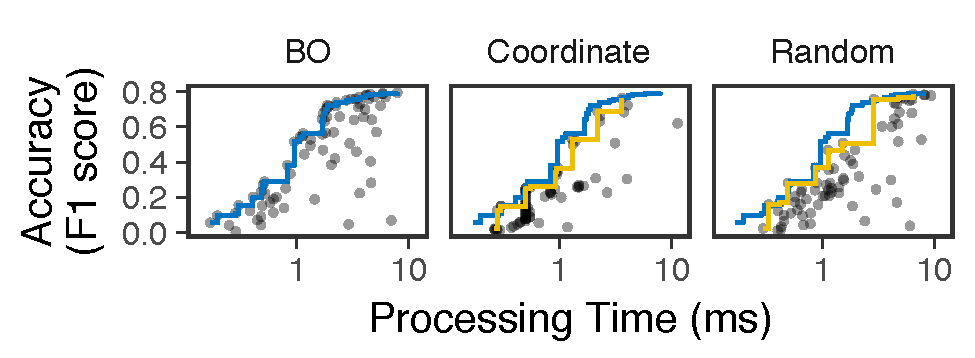
\includegraphics[width=0.85\columnwidth]{figures/bo-eval.pdf}
  \caption{Using Viola-Jones as an example, BO evaluates 50 configurations and
    recommends 29 configurations as the Pareto-optimal boundary (the blue line
    in all subfigures). Greedy and Random find sub-optimal Pareto configurations
    with a budget of 80 evaluations (the yellow line in each figure).}
  \label{fig:bo}
\end{figure}

\subsection{Profile Transfer Across Devices}
\label{sec:performance-transfer}

The profile we learned is specific to the devices. While it seems that we need
to profile for every device, the profiling problem can be simplified. The
insight lies in the properties of our objectives. $A(c)$ doesn't change across
devices. We assume $T(c)$ is monotonic across devices, that is, a slower devices
remains slower for different configurations. Mathematically, if
$T_1(c') < T_1(c)$, then $T_2(c') < T_2(c)$, where $T_1$ and $T_2$ are the
mappings from configurations to processing times on two devices.

As a result, it is easy to see that the same configuration $c$ remains in the
Pareto-optimal set $\mathbb{P}_1$ regardless of what devices the algorithm runs
on. So the whole Pareto-optimal set can be transferred. Visually, the profile on
the second device is a stretched or shrunk version from a reference device along
the dimension of processing times.

This simplifies our performance modeling on a new device as we only need to
measure the new processing times of the Pareto-optimal set. One can even further
reduce the transfer effort by employing a linear transformation: we only need
two measurements about the processing times.

We empirically validate profile transfer on three devices with Viola-Jones face
detector (\autoref{fig:transfer}).

\begin{figure}
  \centering
  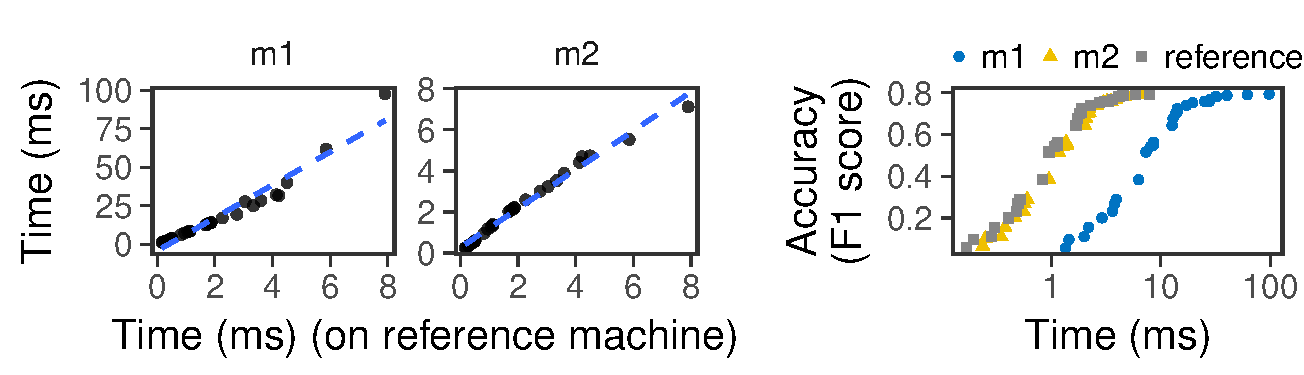
\includegraphics[width=0.9\linewidth]{figures/serving-cross-platform.pdf}
  \caption{(Left) Empirically, processing times follows a linear
    approximation. (Right) Stretched/compressed profile. See paper for
    details.}
  \label{fig:transfer}
\end{figure}


%%% Local Variables:
%%% mode: latex
%%% TeX-master: "../compute"
%%% End:
